\documentclass[11pt,english,a4paper]{article}

\usepackage[utf8]{inputenc}          % Allows UTF-8 encoded characters in the .tex-file.
\usepackage{babel,csquotes,textcomp} % Set LaTeX to structure the content following international academic standards.
\usepackage[titletoc,toc]{appendix}
\usepackage{subfig}

\usepackage{hyperref}
\usepackage{graphicx}
\usepackage{pdfpages}
\usepackage{listings}
\usepackage{wrapfig}
\usepackage{color,colortbl}
\usepackage{lettrine}
\usepackage[font={small,it}]{caption}
\usepackage{multirow}
\usepackage{tabularx}
\usepackage{footnote}
\usepackage{enumitem}
\usepackage{amsmath}

\usepackage{setspace}
\onehalfspacing

\usepackage[
    backend=biber,
    style=numeric
]{biblatex}
\addbibresource{refs.bib}

\lstset{ %
  basicstyle=\ttfamily\small,     
  backgroundcolor=\color{white},   % choose the background color
  breaklines=true,                 % automatic line breaking only at whitespace
  captionpos=b,                    % sets the caption-position to bottom
  commentstyle=\color{mygreen},    % comment style
  escapeinside={\%*}{*)},          % if you want to add LaTeX within your code
  keywordstyle=\color{blue},       % keyword style
  stringstyle=\color{mymauve},     % string literal style
}

\title{Lab report \\ GPSDO}
\author{Aril Schultzen}

\begin{document}
\maketitle
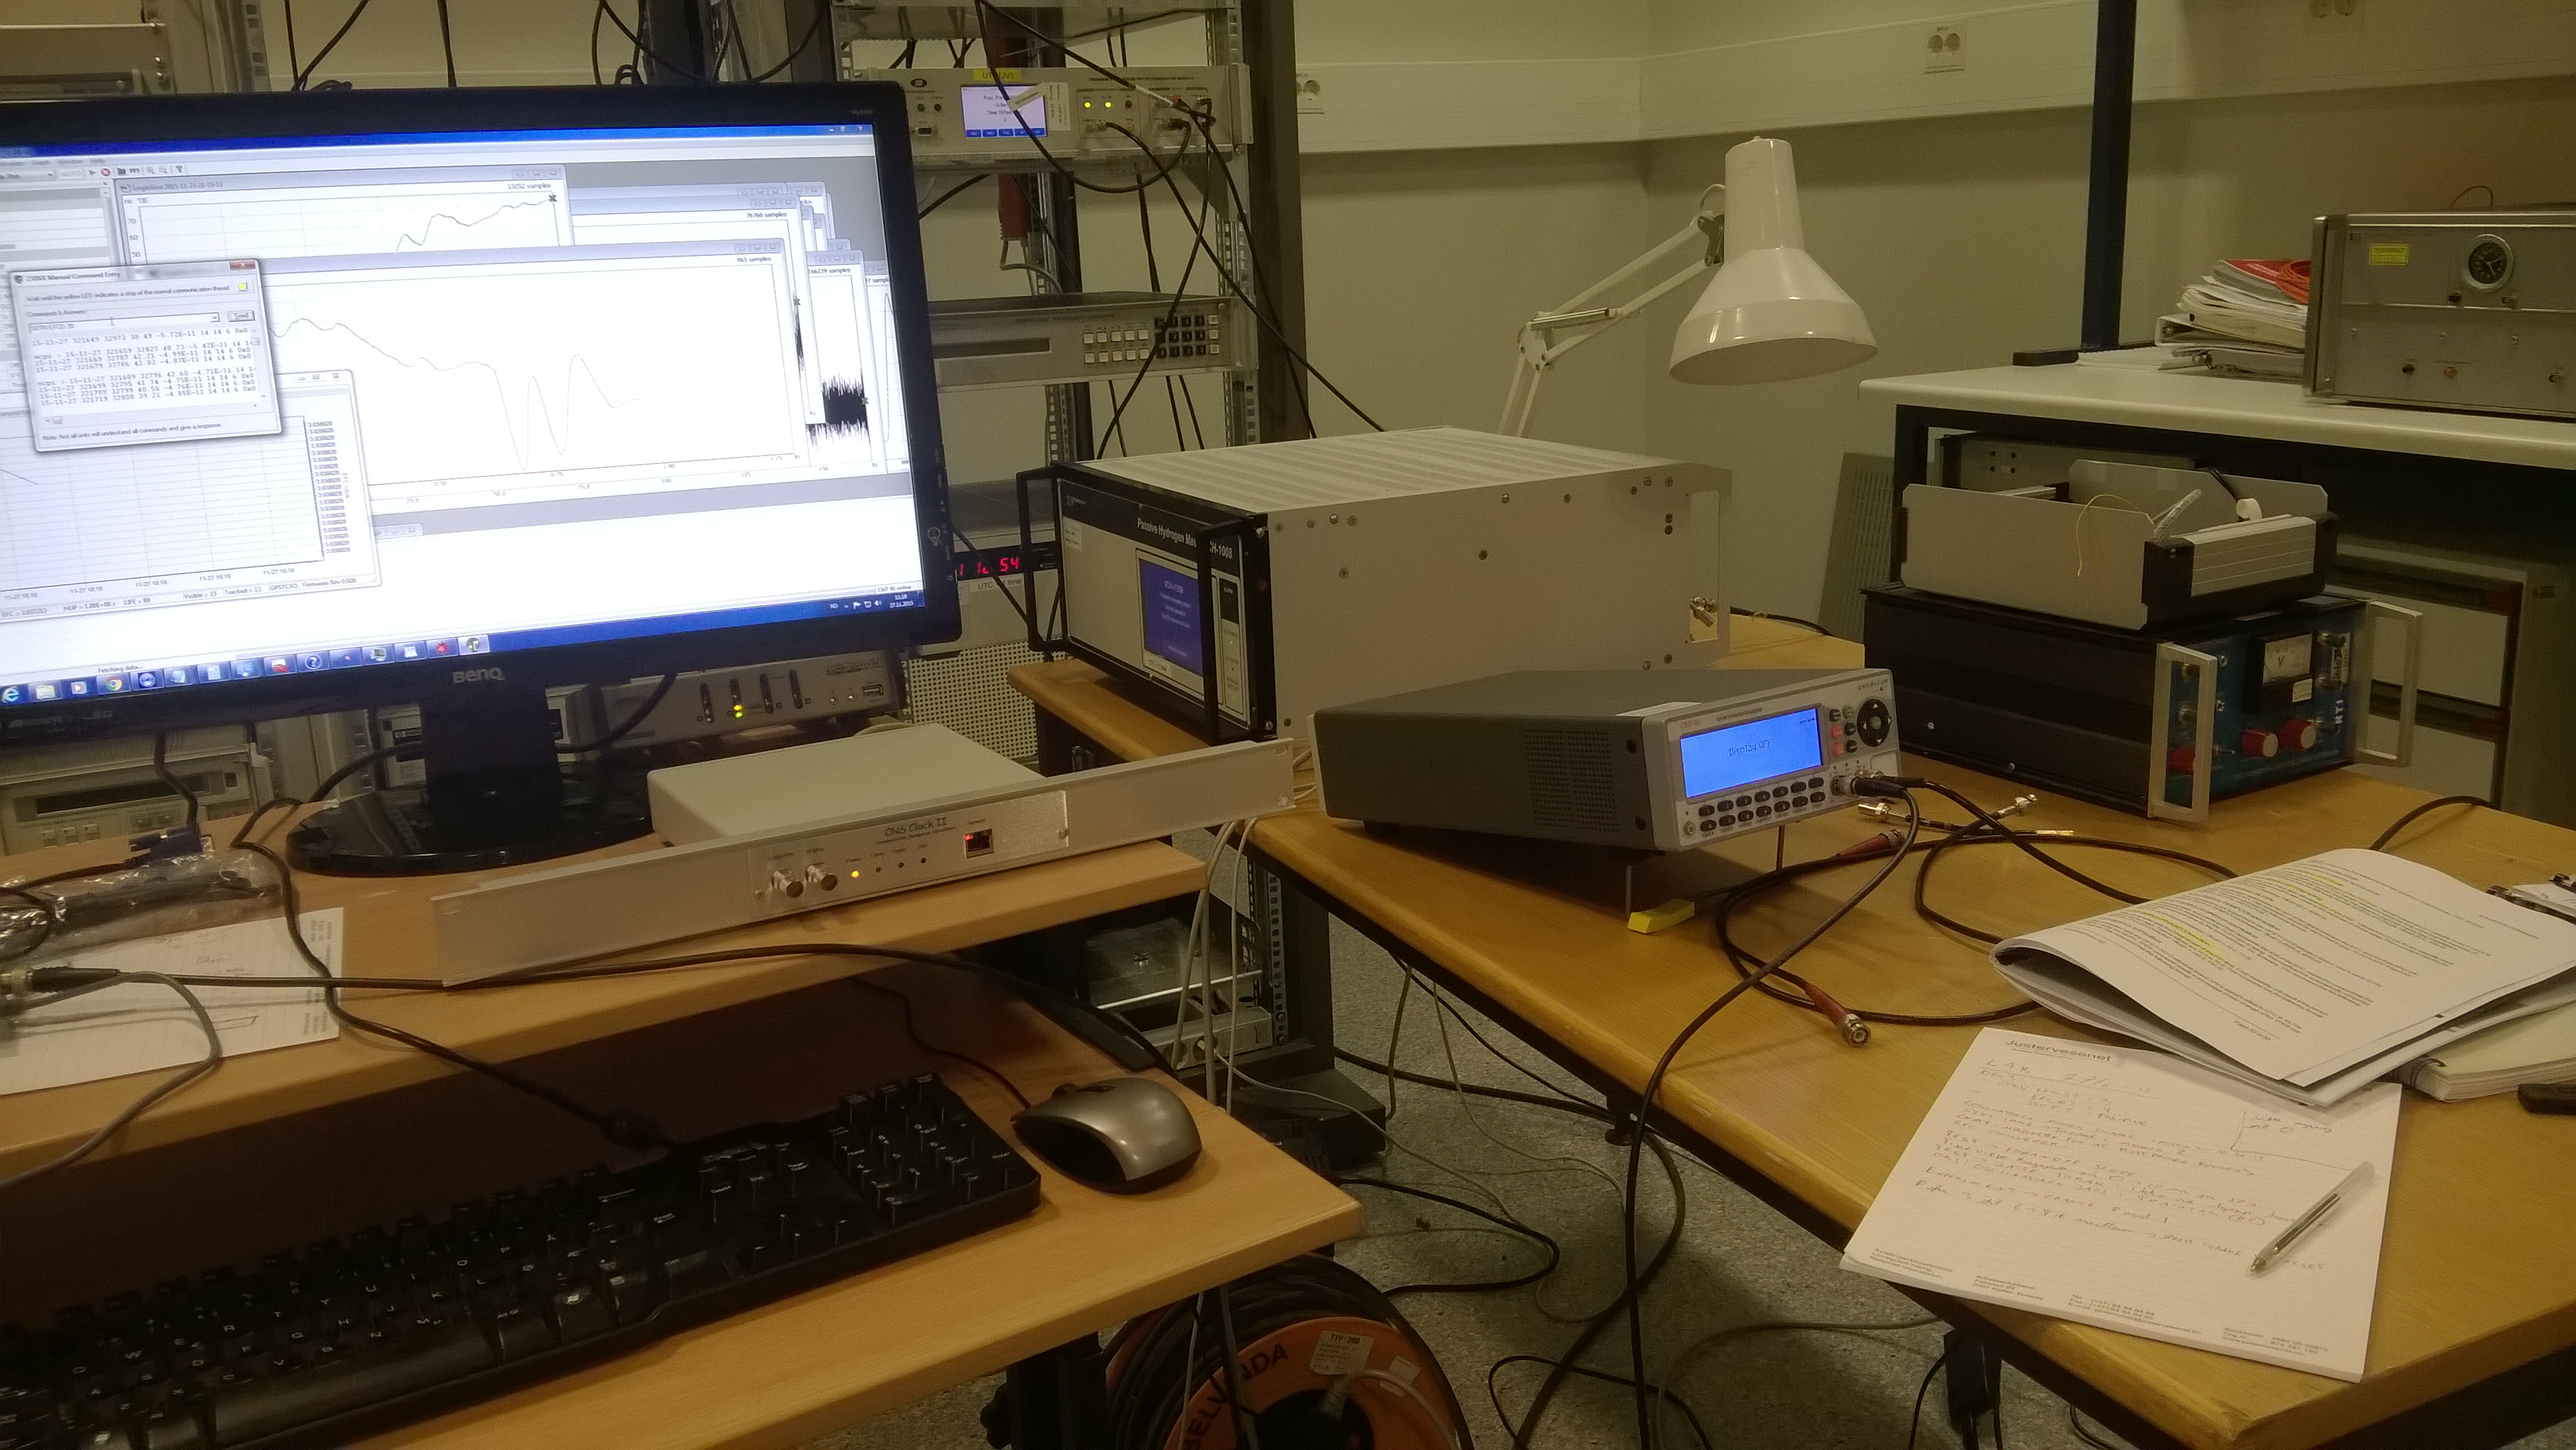
\includegraphics[width=1 \textwidth]{lab.jpg}
\section{Objective}
\begin{itemize}
\item Gain knowledge and understanding of the properties of GPS disciplined oscillator
\item Receive further training in the use of frequency counters as well as tools used to analyze frequency stability.
\end{itemize}

\section{Equipment}
\begin{itemize}
  \item Jackson Labs GPS-300 v1.0 Prototype
  \item PHM, Passive Hydrogen maser, frequency reference
  \item Pendulum CNT-91, Frequency counter
  \item Tektronix MD0-4000-6 Oscilloscope
  \item Z38XX Software
  \item TimeView
  \item TimeLab
\end{itemize}

\section{Before the lab}
\begin{itemize}
  \item The GPS-300 was started in advance and had GPS lock for a minimum of 12 hours.
  \item Z3800X was started and configured to store all log data to the applications root folder with the following format for files: \newline \texttt{Z38XX<YEAR>W<WEEK\_NR>.txt}
  \item A TIE measurement was conducted spanning over 10 hours using the CNT-91 as counter with the maser as reference.
\end{itemize}

\section{Part 1: GPS disciplined oscillator}
\begin{figure}[!htb]
  \centering
  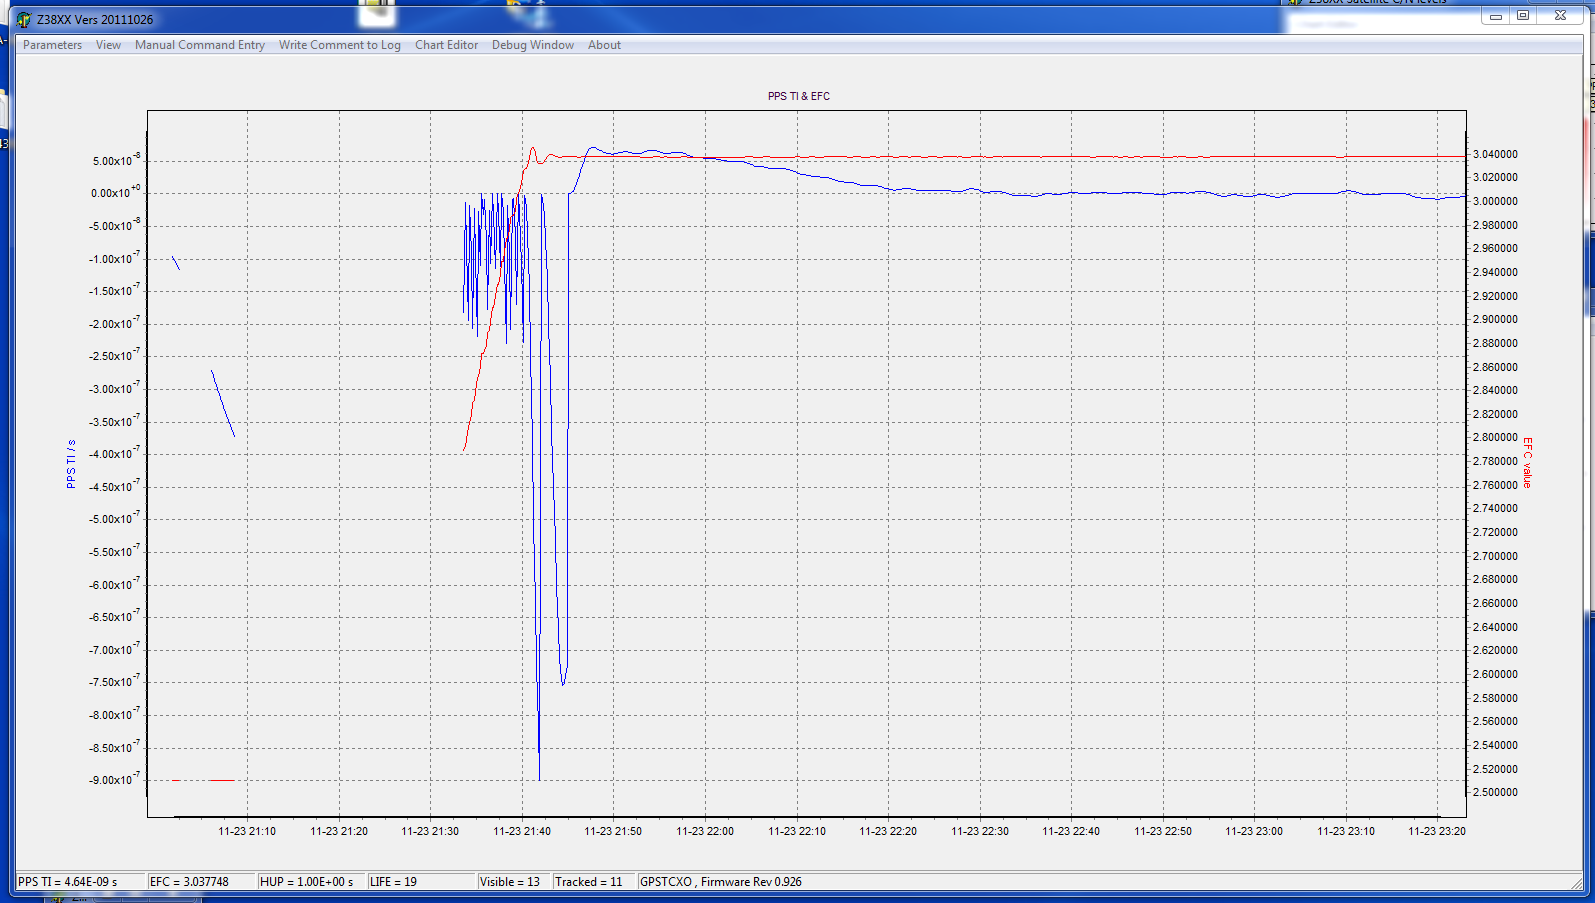
\includegraphics[width=1\textwidth]{z38xx_EFC_oppstart.PNG}
  \caption[Z38XX screen shot] {The figure above shows a screen shot from the Z38XX software. The oscillator is all warmed up and ready to go.} 
  \label{fig:z38xx_oppstart}
\end{figure}

\subsection{Observations}
Figure \ref{fig:z38xx_oppstart} is a screenshot taken from the Z38XX software. The blue plot shows PPS TI (current GPSR time interval difference from UTC or GPS) and the red is the current EFC (Electronic Frequency Control) tuning value. The bar on the bottom of the window shown in the figure, shows that the GPS receiver on the GPS-300 has a total of 13 satellites visible and that it is currently tracking 11, which is more than sufficient for timing purposes. Judging by how stable the EFC have become and how the PPS TI seems to have settled around zero, it is reasonable to assume that the oscillator is warmed up. Note also the fall in EFC in figure \ref{fig:Z38XX_gpsdo12} after we occupied the room and the temperature increased. This increase in temperature has to be compensated for.

\begin{figure}[!htb]
  \centering
    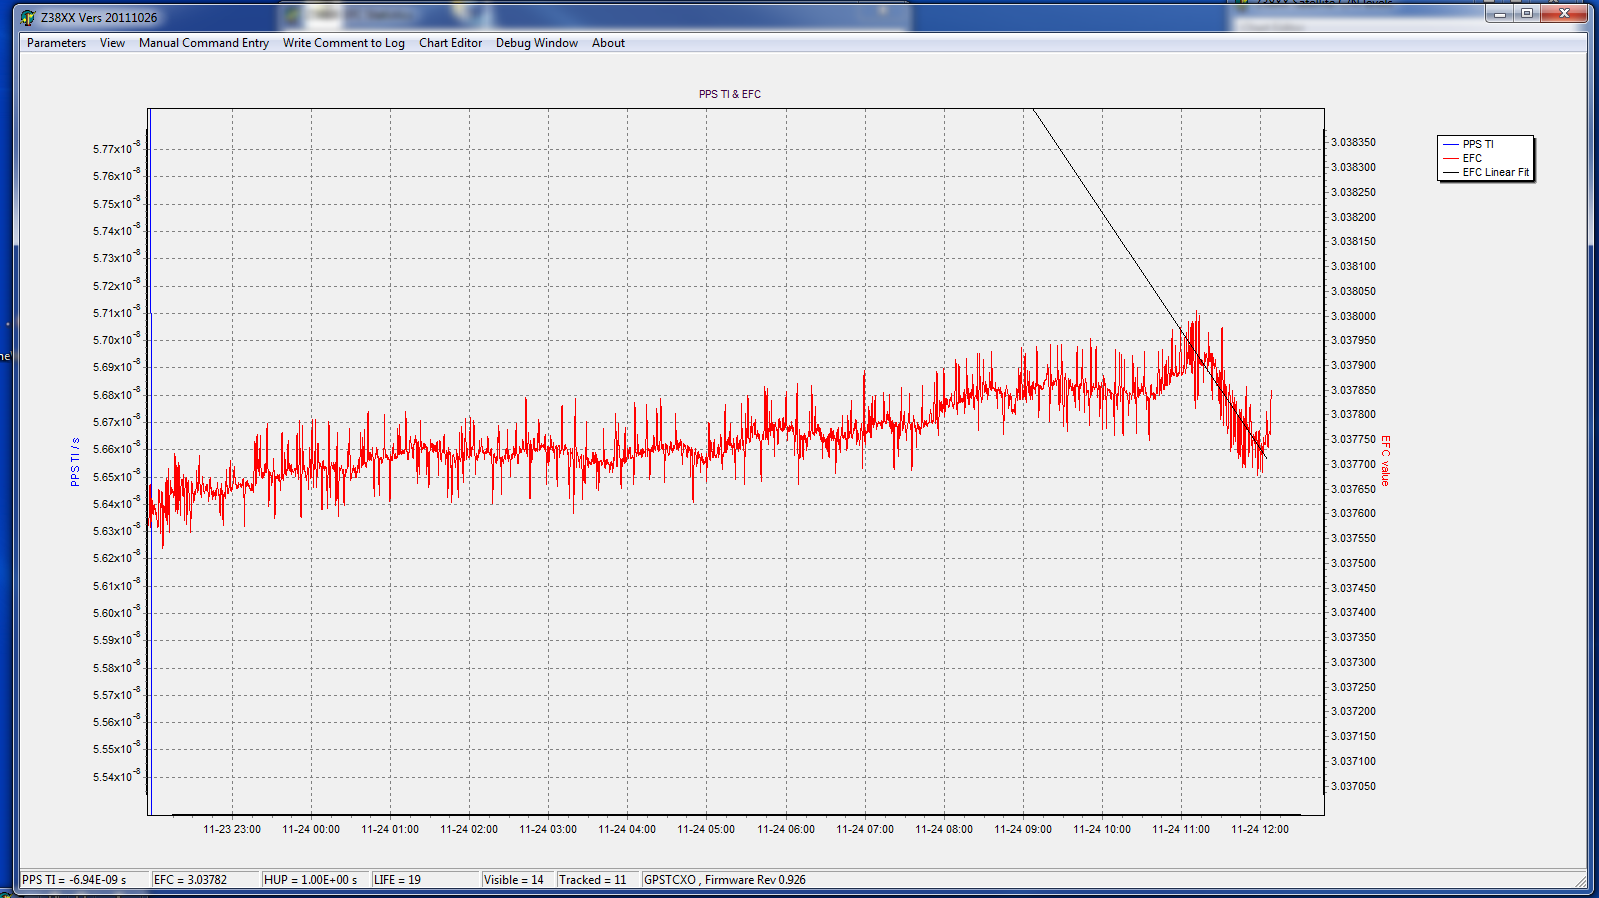
\includegraphics[width=1\textwidth]{z38xx_EFC_oppvarmet_zoom.PNG}
      \caption{Screenshot of Z38XX EFC values since startup. Note the drop towards the end. This is from when we occupied to room and increased the temperature.}
      \label{fig:Z38XX_gpsdo12}
\end{figure}

\begin{figure}[!htb]
  \centering
    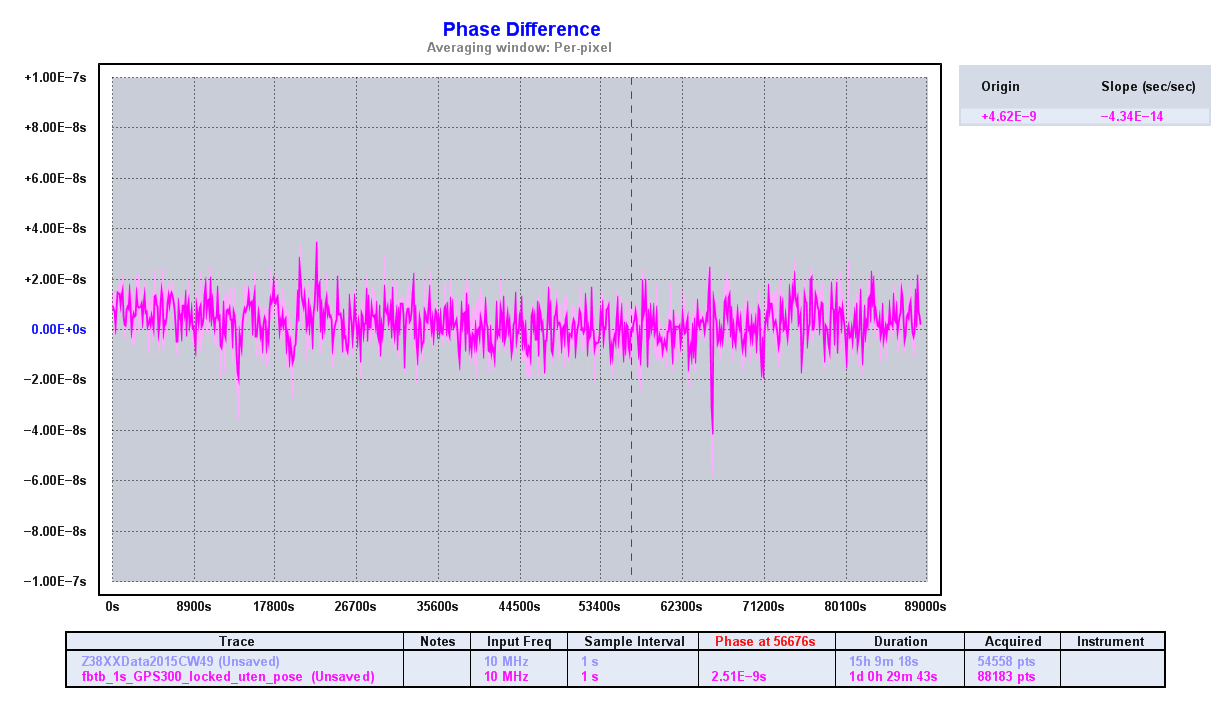
\includegraphics[width=1\textwidth]{part1_spm3_fbtb_phase_diff.png}
      \caption{Phase difference for the GPS-300 measured using the CNT-91 counter}
          \label{fig:part1_spm3_fbtb_phase_diff}
\end{figure}

\begin{figure}[!htb]
  \centering
    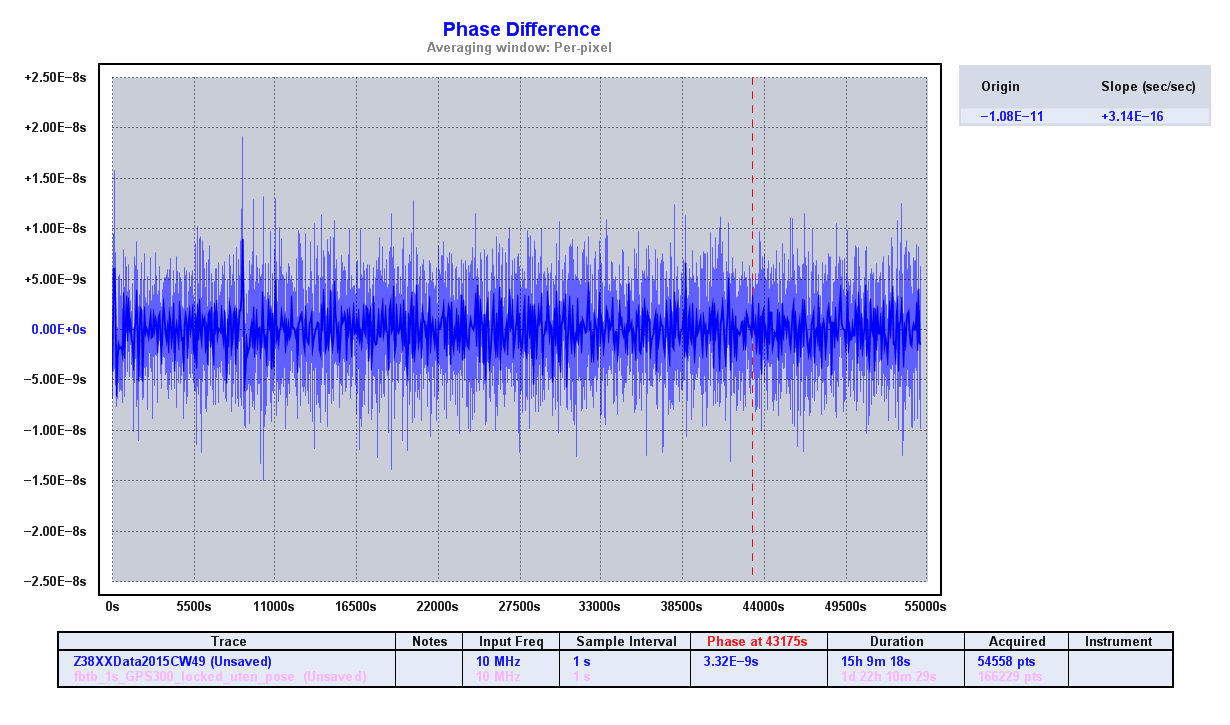
\includegraphics[width=1\textwidth]{part1_spm3_x38_phase_diff.png}
      \caption{Phase difference for the GPS-300 measured using the internal counter}
          \label{fig:part1_spm3_x38_phase_diff}
\end{figure}

When comparing the figure \ref{fig:part1_spm3_fbtb_phase_diff} showing phase difference from a frequency back-to-back  measurement done with our setup and figure \ref{fig:part1_spm3_x38_phase_diff} showing the phase difference measured by the internal counter on the GPS-300, it becomes obvious that there is difference. The measurement made by the counter on the GPS-300 board is more optimistic. The reason for the optimism, is that the GPS-300 is steered towards the GPS signal. Another is that the CNT-91 timer uses the PHM as a 10 MHz reference while the GPS-300 uses 1 PPS from GPS. GPS signals are extremely noisy compared to a PHM and also lack the resolution that the 10 MHz signal offers. The timer on the GPS-300 is also likely sub-par compared to the CNT-91. 

\begin{figure}[!htb]
  \centering
    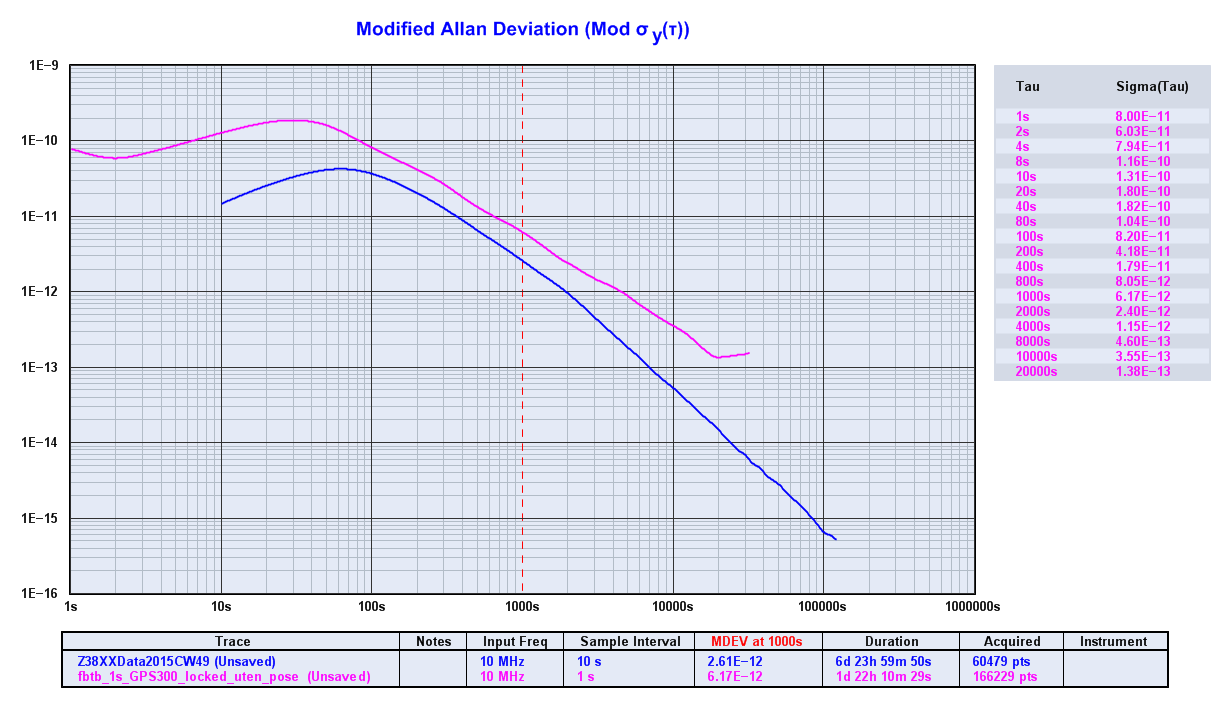
\includegraphics[width=1\textwidth]{part1_spm4_modified_allan.png}
      \caption{Modified Allan Deviation for GPS-300 measured by the internal counter (blue) and CNT-91 (pink)}
          \label{fig:part1_spm4_modified_allan}
\end{figure}

\begin{figure}[!htb]
  \centering
    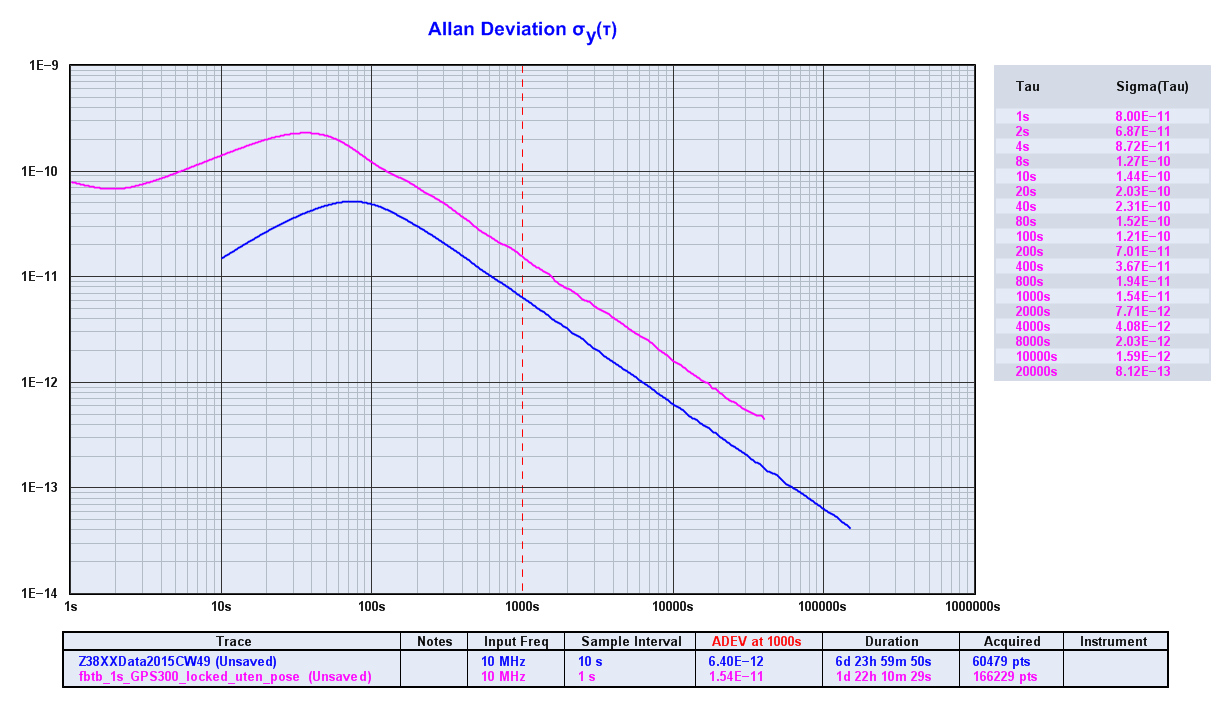
\includegraphics[width=1\textwidth]{part1_spm4_allan.png}
      \caption{Allan Deviation for GPS-300 measured by the internal counter (blue) and CNT-91 (pink)}
          \label{fig:part1_spm4_allan}
\end{figure}

\begin{figure}[!htb]
  \centering
    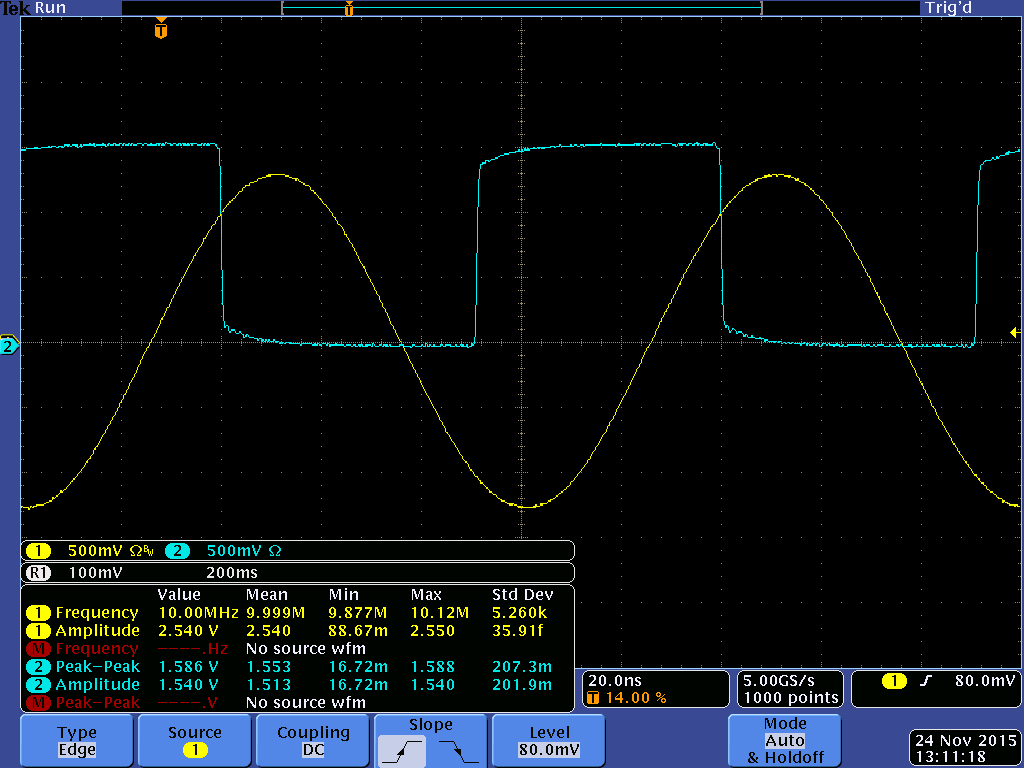
\includegraphics[width=1\textwidth]{tek00006.png}
      \caption{screenshot from the oscilloscope and shows both the GPS-300 and the PHM, trigging at the PHM (yellow)}
          \label{fig:tek00006}
\end{figure}

\begin{figure}[!htb]
  \centering
    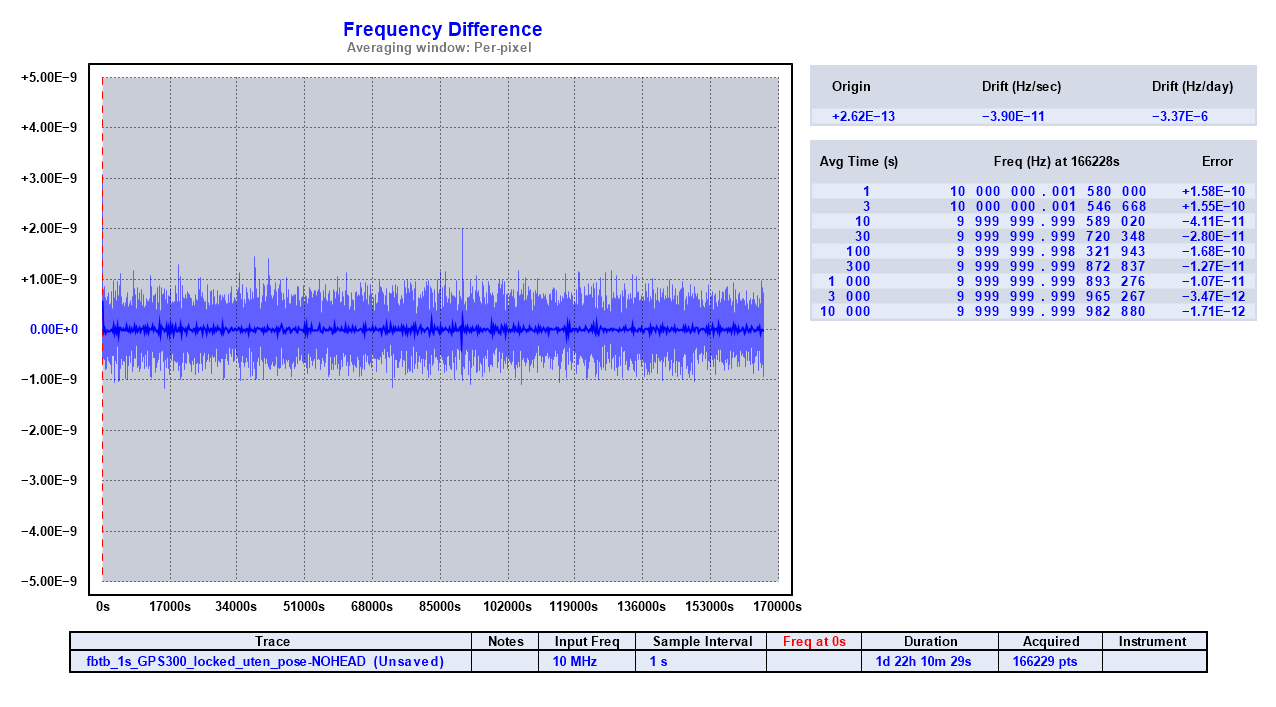
\includegraphics[width=1\textwidth]{part1_spm5_freq_diff.png}
      \caption{GPS-300 1s sample rate frequency back-to-back, frequency difference}
          \label{fig:part1_spm5_freq_diff}
\end{figure}

\newpage
When comparing the measurement done by GPS-300's internal counter with the measurement done by our setup in the context of both regular (figure \ref{fig:part1_spm4_modified_allan}) and Modified Allan Deviation (figure \ref{fig:part1_spm4_allan}), steering, the lack of a high quality reference and counter, results in a incorrect and optimistic measurement (blue plot figure \ref{fig:part1_spm4_modified_allan} and \ref{fig:part1_spm4_allan}) as discussed earlier.  

% spm5 %
Figure \ref{fig:tek00006} is a screenshot of the oscilloscope and shows both the GPS-300 and the PHM, trigging at the PHM (yellow). Upon observation of the oscilloscope, a PID like oscillation effect could be observed. When studying the figure h\ref{fig:part1_spm5_freq_diff} showing the frequency difference made from a measurement done with our setup, this effect becomes more visible. One way to picture it, is that movement along the X-axis on the oscilloscope correlates to "movement" along the the Y-axis on figure \ref{fig:part1_spm5_freq_diff}. 

% spm6 %

\newpage
Figure \ref{fig:del_1_spm6_mod_allan} and \ref{fig:del_1_spm6_allan} shows the Modified and regular Allan Deviation for three measurements all done with our setup:
\begin{itemize}
  \item TIE 100$\mu$s sample rate, PHM (light-blue)
  \item TIE 100$\mu$s sample rate, GPS-300 in holdover mode (red)
  \item TIE 100$\mu$s sample rate, GPS-300 in locked (GPS disciplined mode) smoothed over 1000 points (green)
\end{itemize}
Because of the 1000 point smoothing (green), not much can be said about the stability before 0.1 s. When comparing with the plot for the PHM, it becomes clear that any instability after 0.1 s is not because of the measurement setup, but rather the oscillator itself. However, by using the smoothing method, we are able to obtain resolution that would not be possible because of limitations in the measuring setup, already at 0.1 s instead of $approx$1.6s. By looking at the Modified Allan Deviation for the PHM, the limit of what you could hope to achieve in terms of resolution is revealed. This is because of how the Modified Allan Deviation is calculated by using a running average. This is also what makes it possible to separate white noise from flicker noise since white noise is uncorrelated and therefore possible to reduce by calculating an average.   

Comparing with Symmetricom's own Allan Deviation, the GPS-300 actually performs better than their specifications. At 1 s, we measured 4.42E-11 as opposed to $\approx$ 9.00E-11. At 10 s, we measured 5.20E-11 and they $\approx$6.00E-10.

\begin{figure}[!htb]
  \centering
    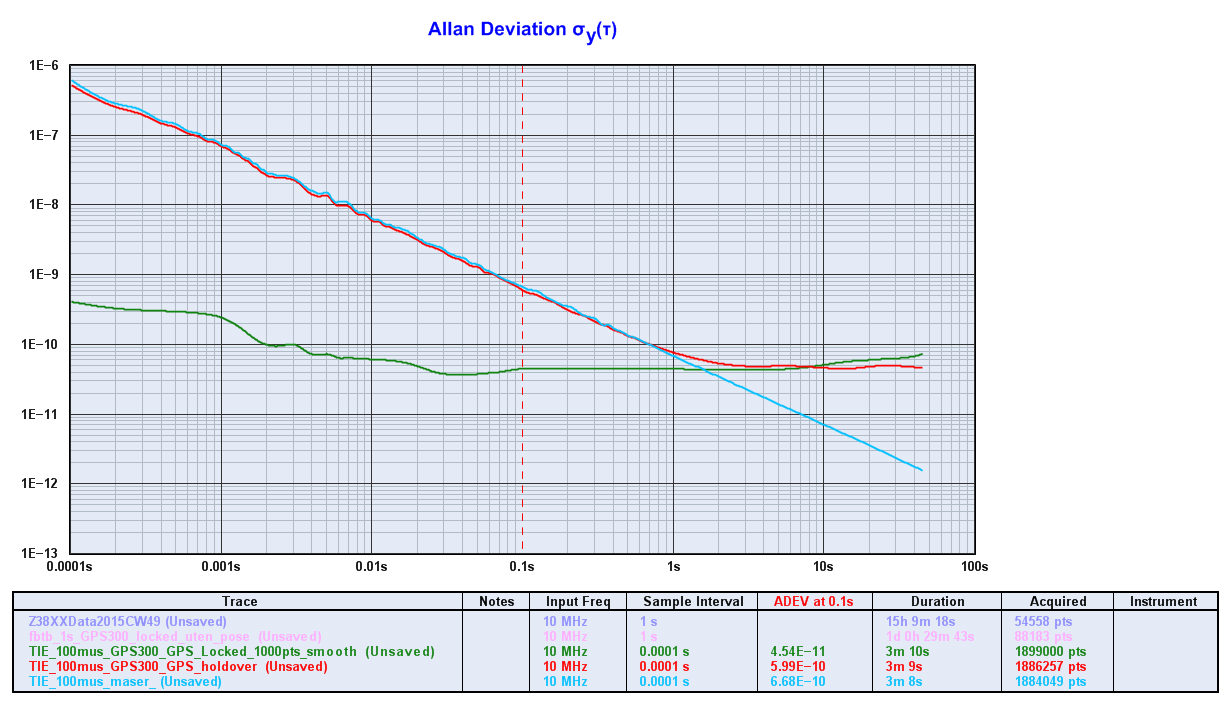
\includegraphics[width=1\textwidth]{del_1_spm6_allan.png}
      \caption{Allan Deviation. TIE 100$\mu$s for GPS-300 in both Locked (green), Holdover (red) and PHM (light-blue). The measurement for Locked GPS-300 is smoothed over 1000 pts.}
          \label{fig:del_1_spm6_allan}
\end{figure}

\begin{figure}[!htb]
  \centering
    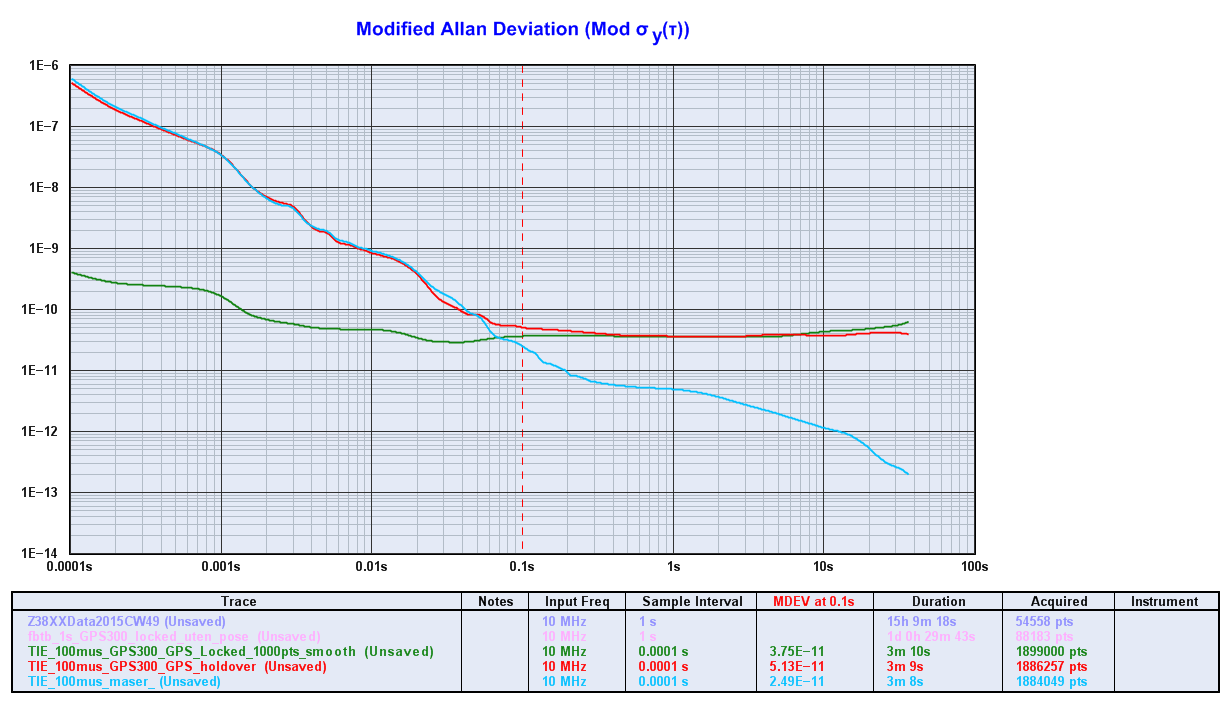
\includegraphics[width=1\textwidth]{del_1_spm6_mod_allan.png}
      \caption{Modified Allan Deviation. TIE 100$\mu$s for GPS-300 in both Locked (green), Holdover (red) and PHM (light-blue). The measurement for Locked GPS-300 is smoothed over 1000 pts}
          \label{fig:del_1_spm6_mod_allan}
\end{figure}

\section{Part 2: Free-range oscillator}

\begin{figure}[!htb]
  \centering
    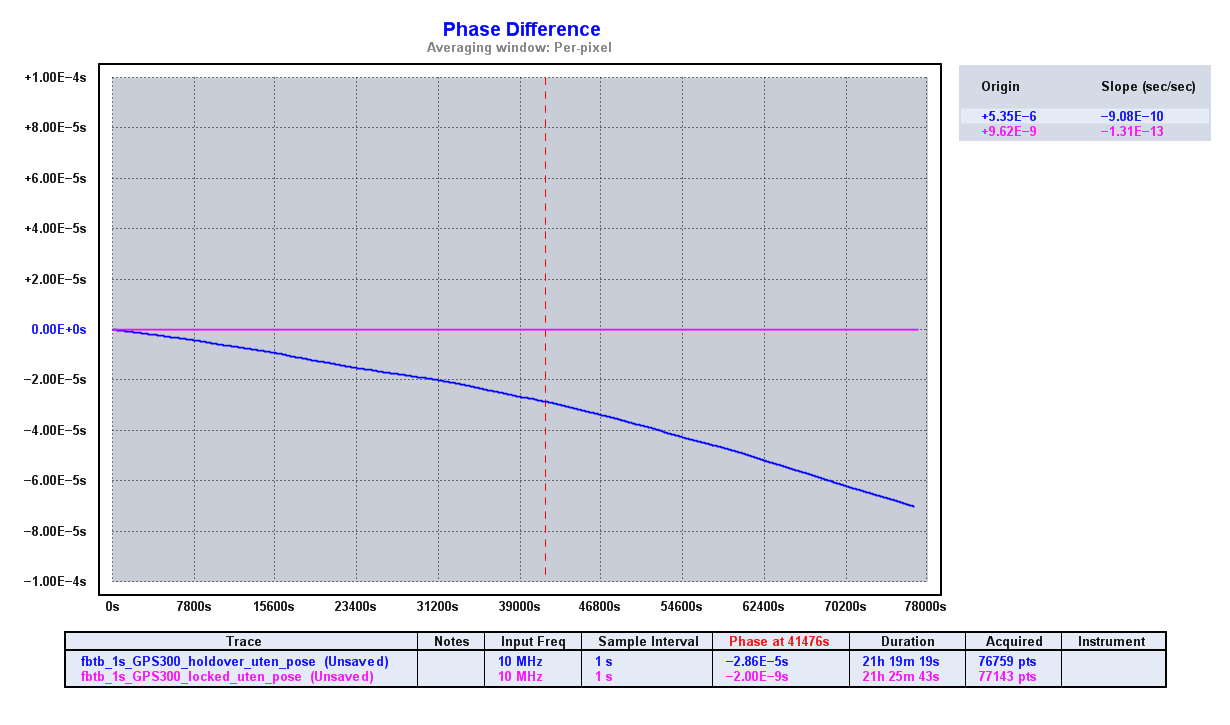
\includegraphics[width=1\textwidth]{del_2_spm1_phase_diff.png}
      \caption{FBTB 1 s, Phase difference for GPS-300 during holdover mode (blue) and locked mode (pink).}
          \label{fig:del_2_spm1_phase_diff}
\end{figure}

\begin{figure}[!htb]
  \centering
    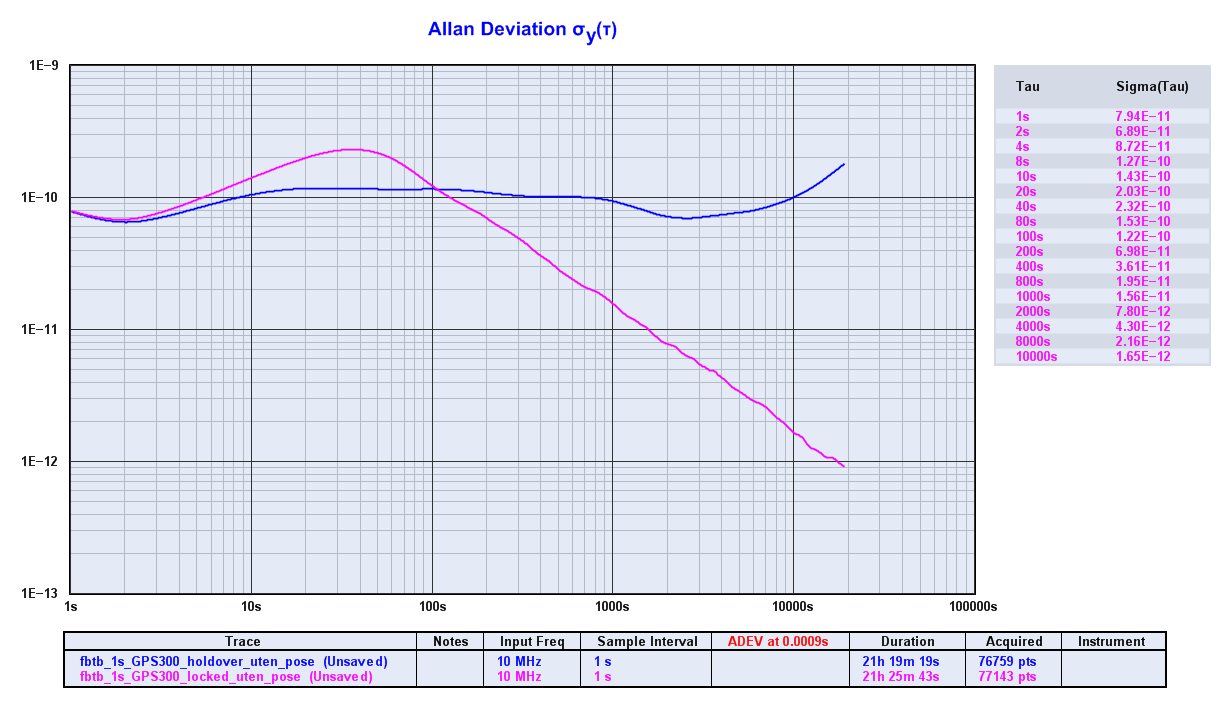
\includegraphics[width=1\textwidth]{del_2_spm1_allan_dev.png}
      \caption{FBTB 1 s, Allan Deviation for GPS-300 during holdover mode (blue) and locked mode (pink).}
          \label{fig:del_2_spm1_allan_dev}
\end{figure}
When comparing the Allan Deviation for the measurement taken with and without GPS lock (figure \ref{fig:del_2_spm1_allan_dev}), one can observe that the long term stability is better when in locked mode. This is not a surprise, but when observing the plot for the oscillator when in Holdover mode, one can see that the short term stability is better than when disciplined. One could perhaps argue that the oscillator short term stability in locked mode would benefit from a longer time constant (between GPS synch), but this depends on the temperature variations of the environment of which it is operating. In the lab where this experiment was exercised, the temperature is much more stable than one could hope to encounter "in the wild".

\begin{figure}[!htb]
  \centering
    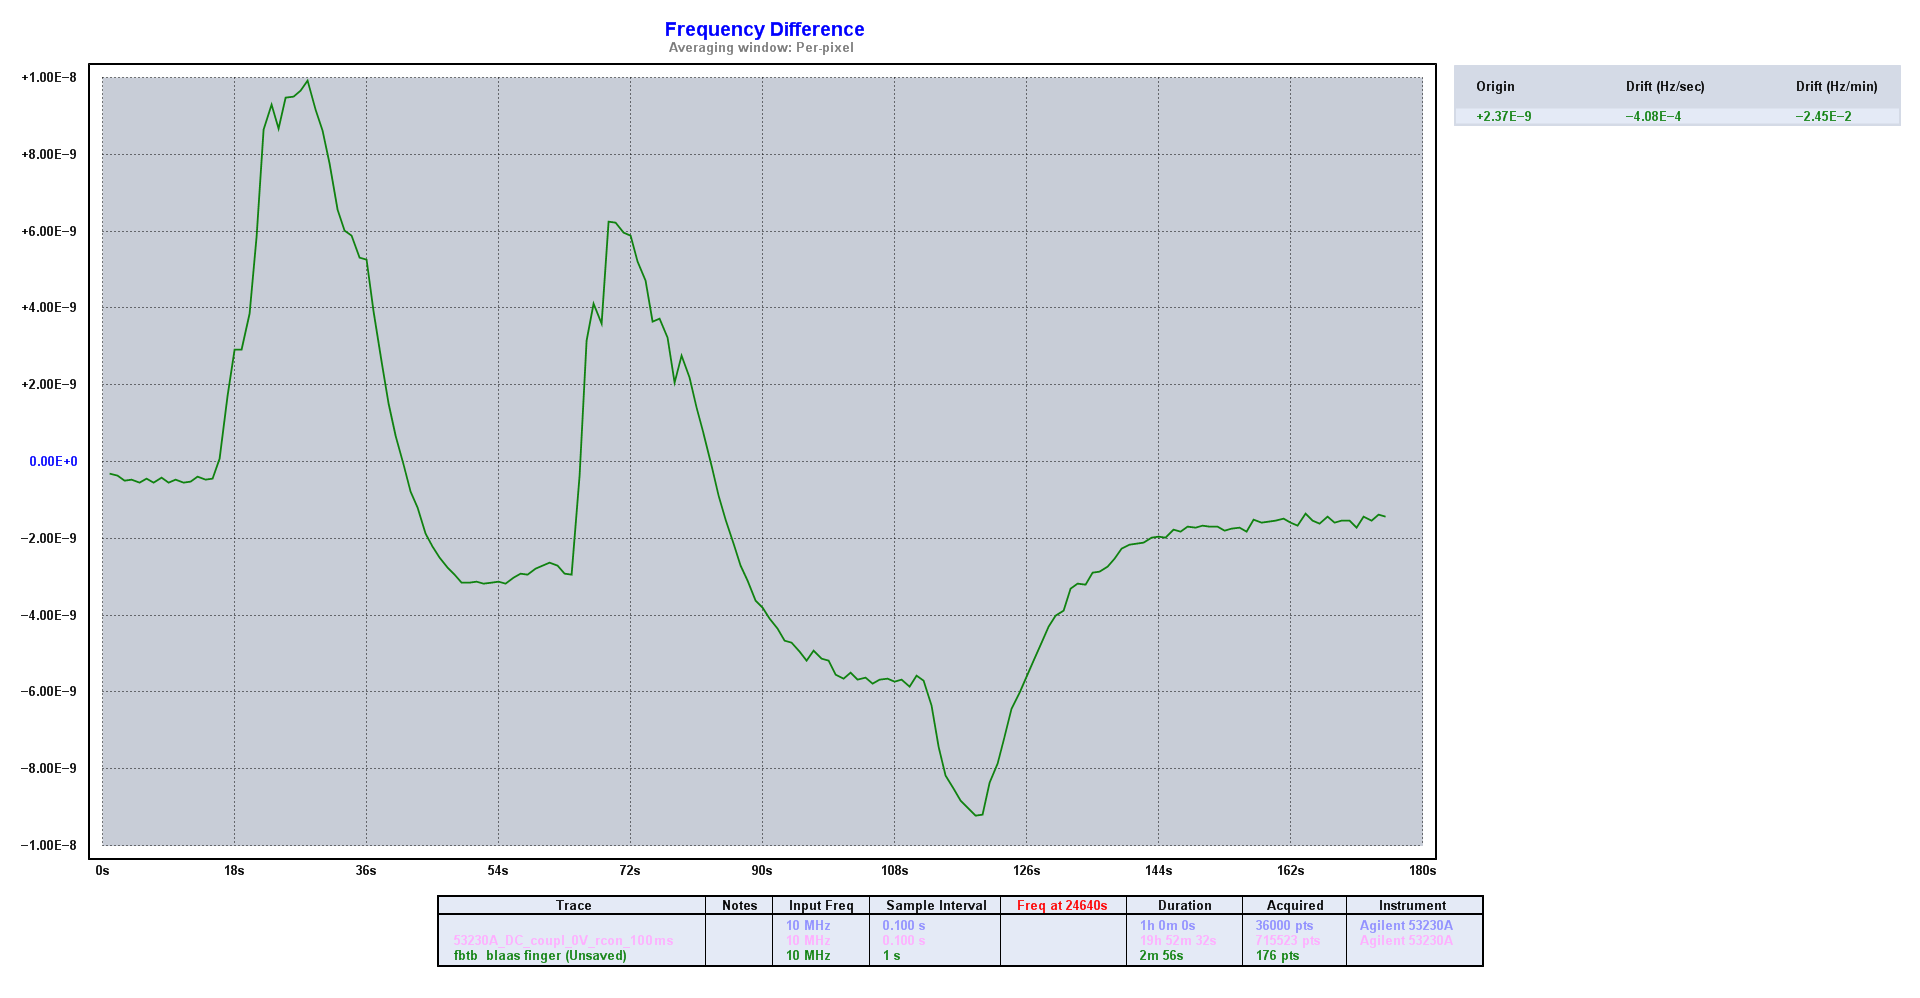
\includegraphics[width=1\textwidth]{del_2_spm2_fbtb_blaas_finger.png}
      \caption{Figure is showing variance in frequency from heating up and cooling down the oscillator by touching and blowing on it.}
          \label{fig:del_2_spm2_fbtb_blaas_finger}
\end{figure}

Figure \ref{fig:del_2_spm2_fbtb_blaas_finger} shows what happens when you heat the oscillator up or cool it down. The first peak is when i put my finger on it and and the dip is when i blew air on it. The next peak and dip is from the same, but now the temperature compensation seems to have picked up the change, hence the last deep dip. The bottom-line is that the frequency increases as temperature drops and frequency decreases as temperature rises. 
After putting GPS-300 into holdover mode which means it is no longer disciplined by the GPS chip on the board, i measured it going from holdover and into locked mode using both out setup, (figure \ref{fig:del_2_spm3_fra_holdover_to_locked}) and the internal counter (figure \ref{fig:del_2_spm3_fra_holdover_to_locked_z38}). Unfortunately, there is an error in the figure \ref{fig:del_2_spm3_fra_holdover_to_locked} where the wrong sample interval has been used. It should have been 10 s instead of 1. However, it still shows how the internal counter has been a little optimistic as mentioned earlier. 

\begin{figure}[!htb]
  \centering
    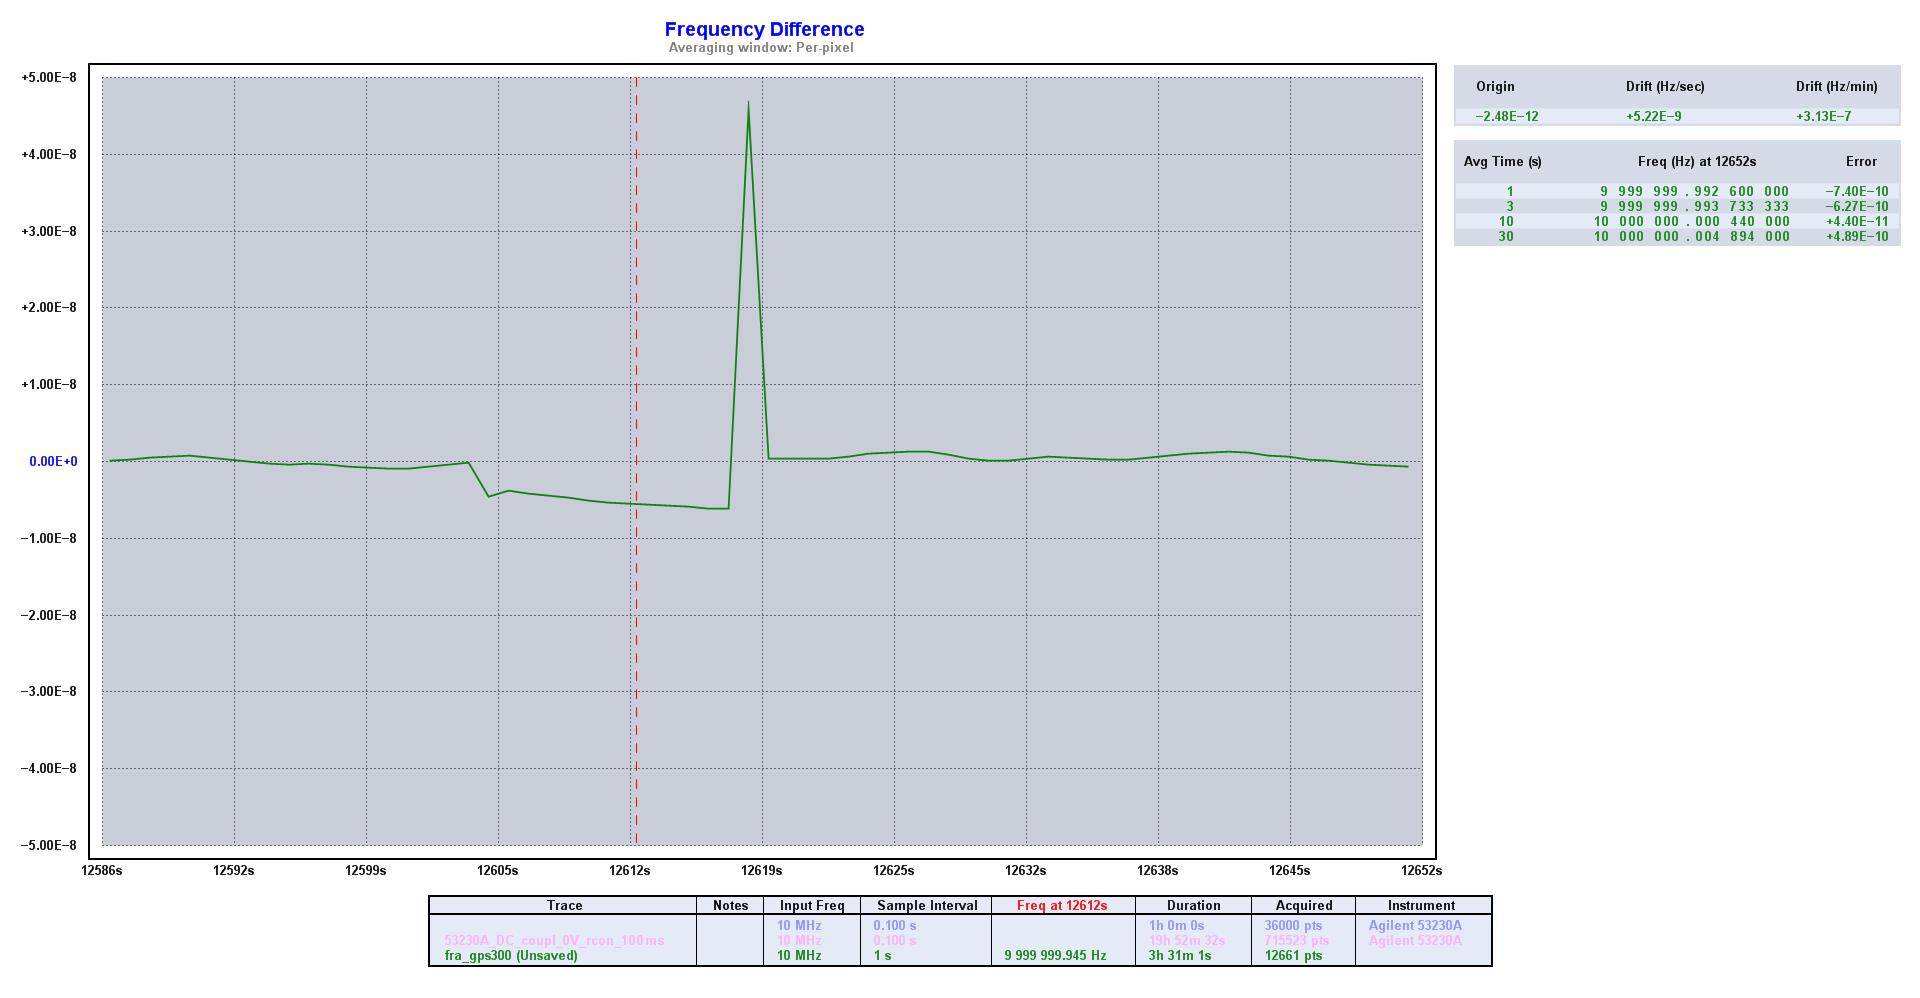
\includegraphics[width=1\textwidth]{del_2_spm3_fra_holdover_to_locked.png}
      \caption{Figure is showing GPS-300 going from holdover mode to locked. Measurement was made by CNT-91 frequency counter. Note! The presentation of this measurement in TimeLab is made using the wrong sample interval, it should be 10s and not 1s. This only affects the x axis.}
          \label{fig:del_2_spm3_fra_holdover_to_locked}
\end{figure}

\begin{figure}[!htb]
  \centering
    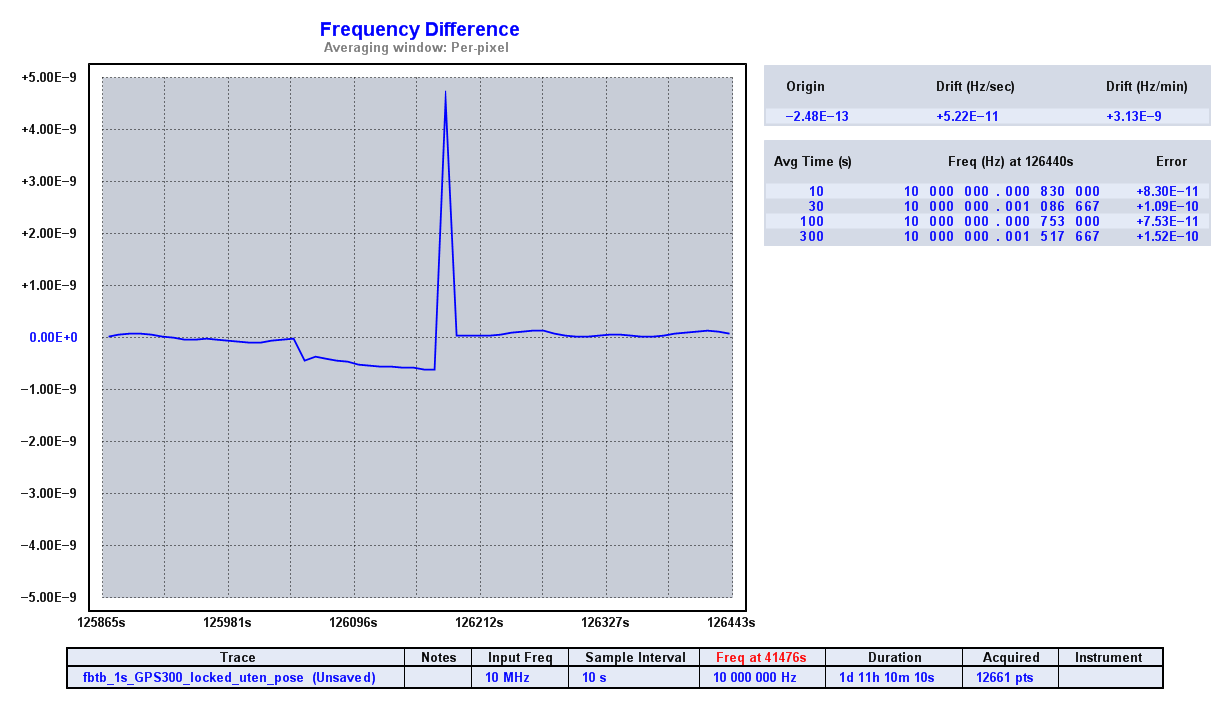
\includegraphics[width=1\textwidth]{del_2_spm3_fra_holdover_to_locked_z38.png}
      \caption{Figure is showing GPS-300 going from holdover mode to locked. Measurement was made by the internal counter on GPS-300.}
          \label{fig:del_2_spm3_fra_holdover_to_locked_z38}
\end{figure}


\section{Part 3: Stability parameters}
The GPS-300 GPSTXO has a set of parameters related to it's PID loop. By adjusting these parameters, the PID can be adjusted or tuned. When i was experimenting with stability parameters, i discovered (not surprisingly) that some of the parameters had a greater effect than others. In hindsight it's pretty obvious that i should have experimented a little more with the PHASECO and EFCD and perhaps have tried different values in order to provoke the typical response for that part of parameter. The values was set back to default between each measurement and the unit was in Locked mode the whole time. A base line is included in all the figures. This baseline is just a measurement done prior to the experimenting.

\subsection{EFCS}
The EFCS parameter is the proportional part of the PID loop. It is according to the manual typically set between 0.7 to 6.0. Figure \ref{fig:EFCS} shows what happens when it was set to 20. When proportional gain is set this high, it overshoots dramatically and begins to oscillate.

\begin{figure}[!htb]
  \centering
    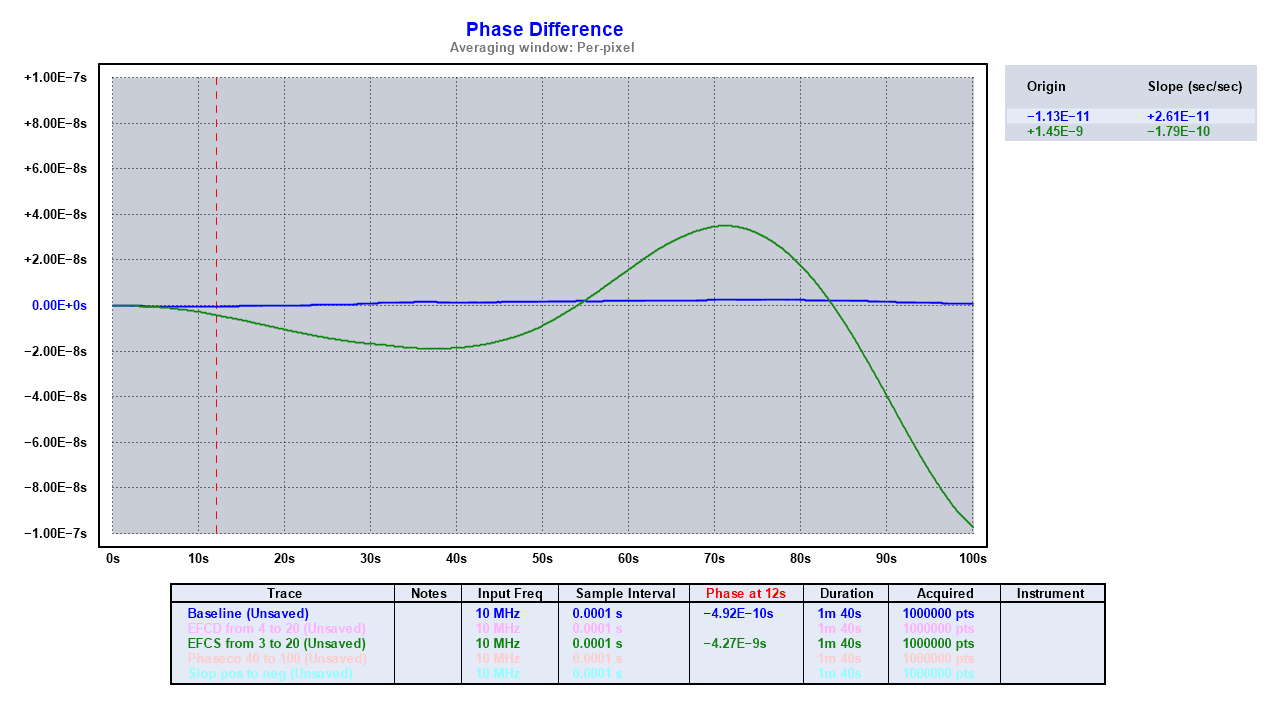
\includegraphics[width=1\textwidth]{EFCS.png}
      \caption{TIE 100$\mu$s sample rate 100s total, phase difference for base line (blue) and for when stability parameter EFCS = 20}
          \label{fig:EFCS}
\end{figure}

\subsection{PHASE}
The PHASECO sets the Integral part of the PID loop. I set it to 100 and made the measurement as seen in figure \ref{fig:PHASE}. Typical values are between 10 and 30. Since it is set so high, it overshoots and restricts the loop from reaching the set point. 

\begin{figure}[!htb]
  \centering
    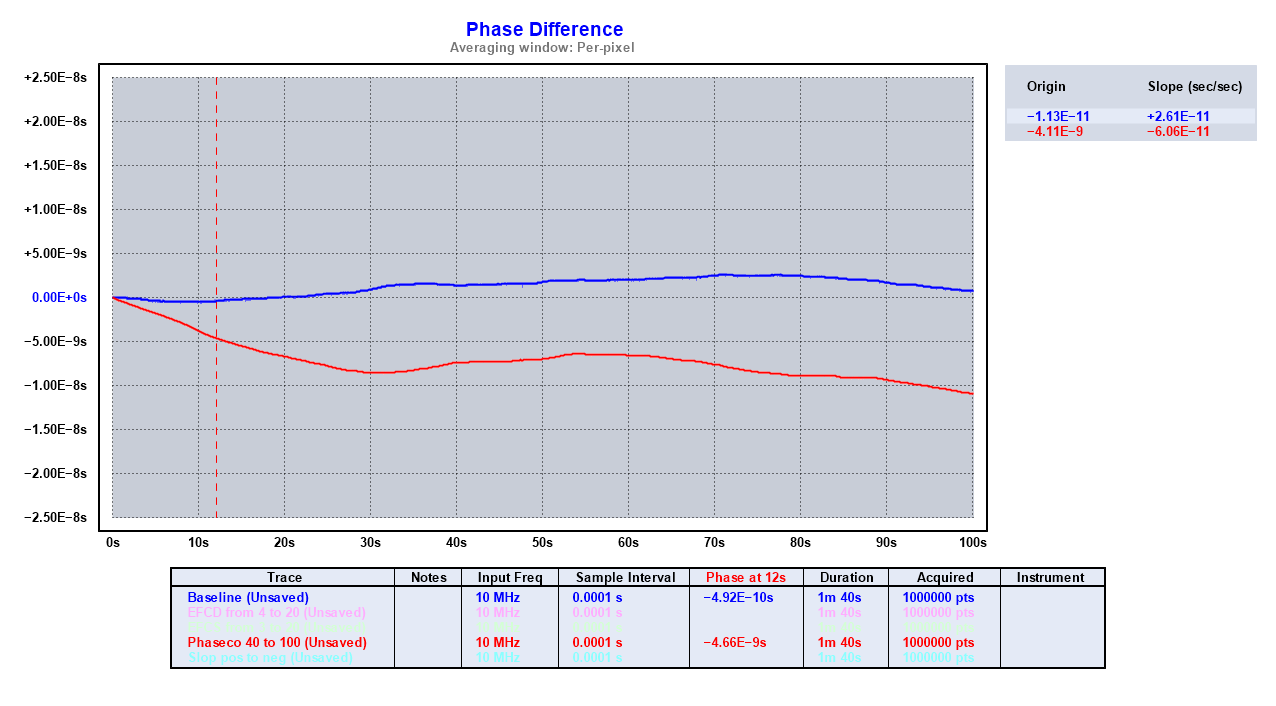
\includegraphics[width=1\textwidth]{PHASE.png}
      \caption{TIE 100$\mu$s sample rate 100s total, phase difference for base line (blue) and for when stability parameter PHASECO = 100}
          \label{fig:PHASE}
\end{figure}

\subsection{EFCD}
The EFCD is the Dampening part of the PID loop. I set it to 20 and made the measurement as seen in figure \ref{fig:EFCD}. If the P part (EFCS) of the PID had been set higher, the effect might have been more visible. The noise seemed to be decrease compared to the base line.

\begin{figure}[!htb]
  \centering
    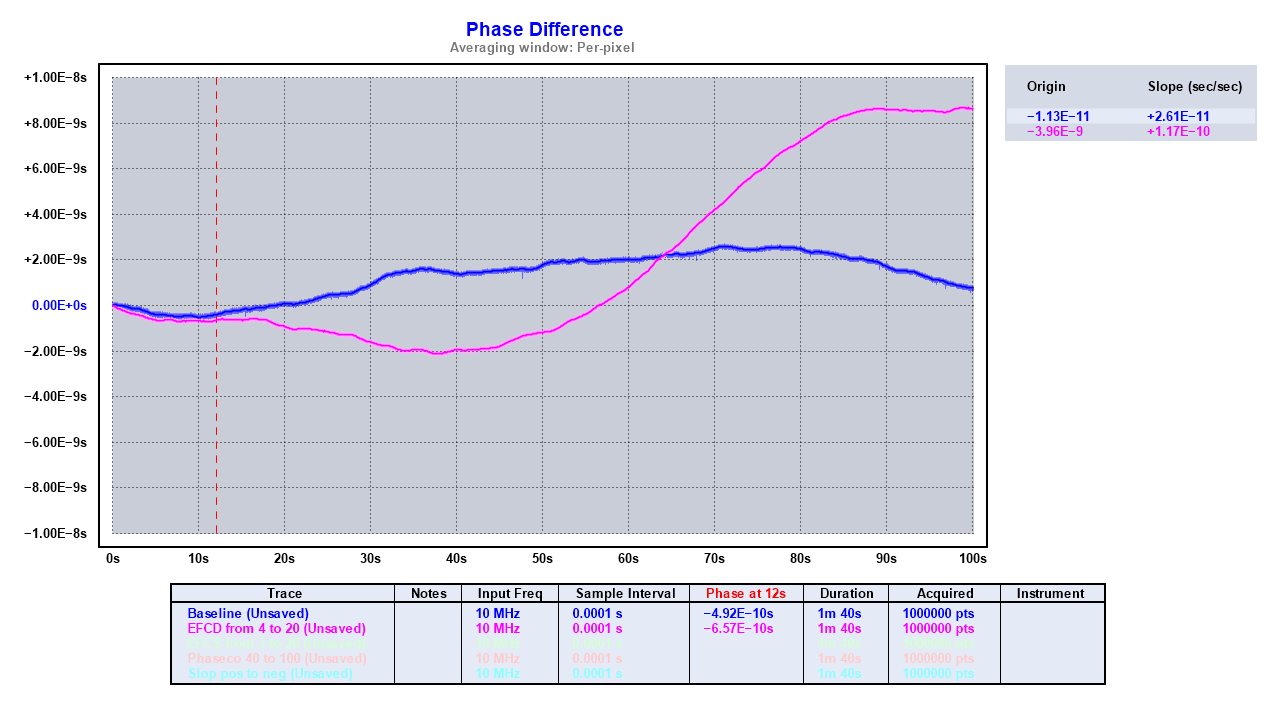
\includegraphics[width=1\textwidth]{EFCD.png}
      \caption{TIE 100$\mu$s sample rate 100s total, phase difference for base line (blue) and for when stability parameter EFCD = 20}
          \label{fig:EFCD}
\end{figure}

\subsection{SLOP}
Not strictly part of the PID. The SLOP sets the sign of the slope between the EFC and the TCXO's frequency variation. By default, it's set to positive. Setting it to negative will completely wreck the stability of the oscillator in a very short time. When the loop tries to counter an error but applies a correction with the wrong slope, the error will become worse and worse for every correction. No matter how hard the loop tries to fix the error, it will only get worse since the sign is wrong. 

\begin{figure}[!htb]
  \centering
    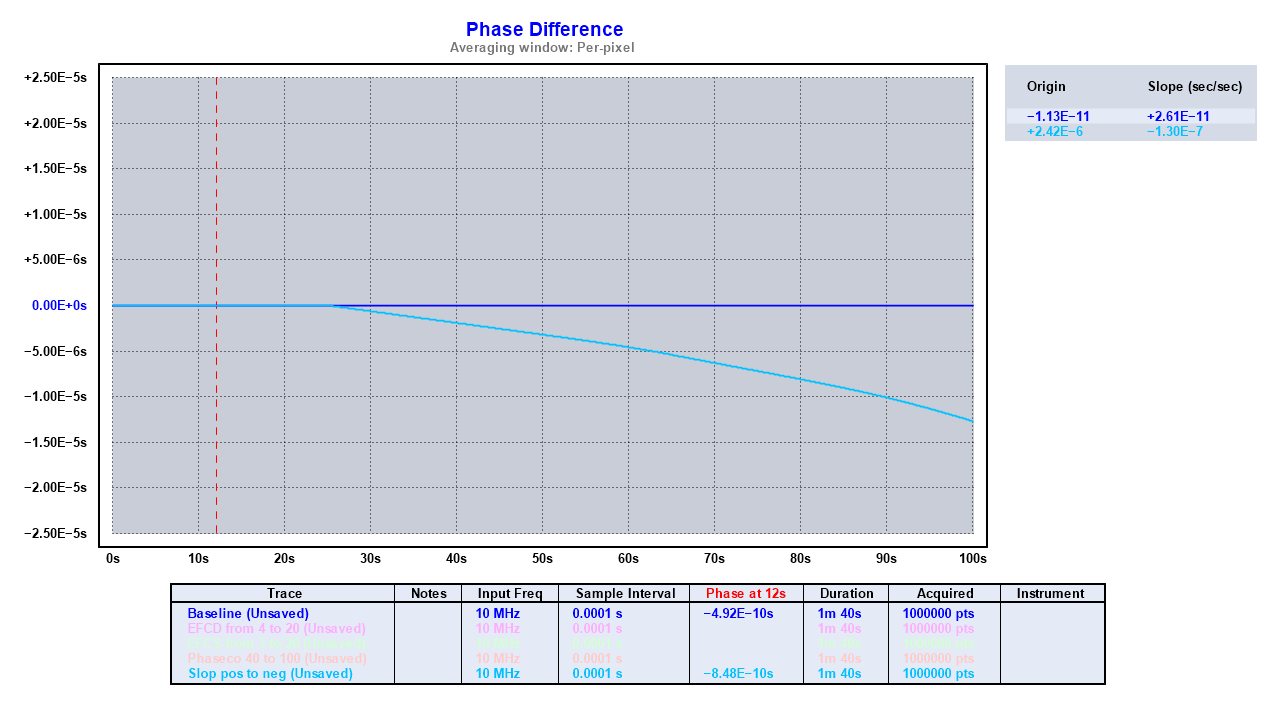
\includegraphics[width=1\textwidth]{SLOP.png}
      \caption{TIE 100$\mu$s sample rate 100s total, phase difference for base line (blue) and for when stability parameter SLOP = NEG}
          \label{fig:SLOP}
\end{figure}





\end{document}                     